\documentclass[hidelinks, 12pt, a4paper]{article}

\usepackage{tabularx} %full-width tables
\usepackage{moresize} %Huge and HUGE
\usepackage[margin=0in]{geometry}%Margins
\usepackage[none]{hyphenat}%Remove hyphenation
\usepackage{enumitem}%to set gaps in itemize
\usepackage{fontawesome}
\usepackage{hyperref}
\usepackage{blindtext}
\usepackage{xcolor}
\usepackage{afterpage}
\usepackage{tikz}
\usepackage[skins]{tcolorbox}
\usepackage{xcolor}

\usepackage{multicol}

\usepackage[sfdefault,light]{roboto}

%\cellwidth in tabularx size
\makeatletter
\newcommand\cellwidth{\TX@col@width}
\makeatother

\definecolor{sidebarColor}{HTML}{001C5E}
\definecolor{skillBackground}{HTML}{98A0B2}
\definecolor{skillForeground}{HTML}{EBA500}

%Right-aligned tabularx
\newcolumntype{R}{>{\raggedleft\arraybackslash}X}

%No page numbering
\pagenumbering{gobble}

\newcommand{\smitem}[1]{\item {\small {#1}}}

\newenvironment{bullets}{\begin{minipage}[t]{\linewidth}\begin{itemize}[leftmargin=2em,label=-,nosep]}{\end{itemize}\end{minipage}\vspace{2pt}}

\newenvironment{sectionitem}{\vspace{6pt}\noindent\tabularx{\linewidth}{p{70pt}X}}{\endtabularx}

\newcommand{\tech}[1]{
	\tcbox[skin=enhanced,nobeforeafter,colframe=black!20,size=fbox,height=15pt]{\footnotesize#1}
}

\newcommand{\darktech}[1]{
	\tcbox[skin=enhanced,nobeforeafter,colback=black!10,colframe=black!30,size=fbox,height=15pt]{\footnotesize#1}
}

\newcommand{\sectionheader}[1]{
	\vspace{6pt}
	{
		\noindent
		\hspace{3pt}
		%\fontfamily{lmr}\selectfont
		\Large\textbf{#1}}}

\begin{document}
	\noindent\fcolorbox{sidebarColor}{sidebarColor}{%
		\color{white}
		\begin{minipage}{\dimexpr0.35\textwidth-2\fboxrule-2\fboxsep\relax}
			\vspace{4pt}
			\begin{center}
				\begin{tikzpicture}
				\color{black}
				\node[circle,draw,inner sep=40pt,fill overzoom image=picture] (A) {};
				\end{tikzpicture}\\
				
				\vspace{12pt}
				
				\textbf{
					\LARGE Steven Waterman
				}
				\vspace{8pt}
				
				\begin{tabular}{rc}
					Durham, UK                                                     & \faHome                                                       \\
					\href{mailto:cv@stevenwaterman.uk}{cv@stevenwaterman.uk}           & \href{mailto:cv@stevenwaterman.uk}{\faEnvelope}                 \\
					\href{https://www.linkedin.com/in/steven-waterman/}{steven-waterman} & \href{https://www.linkedin.com/in/steven-waterman/}{\faLinkedin} \\
					\href{https://github.com/stevenwaterman}{StevenWaterman}       & \href{https://github.com/stevenwaterman}{\faGithub}           \\
					\href{https://twitter.com/SteWaterman}{SteWaterman}       & \href{https://twitter.com/SteWaterman}{\faTwitter}           \\
					\href{http://www.stevenwaterman.uk}{stevenwaterman.uk}             & \href{http://www.stevenwaterman.uk}{\faLink}                    \\
				\end{tabular} \\
				
				\vspace{4pt}
				
				\begin{minipage}{0.9\linewidth}
					\begin{center}
						\begin{Large}
							\textbf{Summary}
						\end{Large}
					\end{center}
				
					\vspace{-8pt}
					
					Full-Stack Developer at Scott Logic
					
					\vspace{8pt}
					
					Self-directed, efficient generalist, able to quickly learn new technologies with a desire to work on challenging problems
					
					\vspace{8pt}
					
					Creative, unorthodox, innovative. Able to think outside the box to find the best solution
					
					\vspace{8pt}
					
					Thought leader, giving frequent tech talks and maintaining an active blogging presence
					
					\vspace{8pt}
					
					Back-end and Data Infrastructure focus. While I'm happy to work on the behind-the-scenes of front-end, this CV is my artistic peak!
					
					\vspace{4pt}
					
					\begin{center}
						\begin{Large}
							\textbf{Career Interests}
						\end{Large}
					\end{center}
				
					\vspace{-8pt}
					
					Startups and small teams with flat hierarchy, in North-East England or (ideally) Remote.
					
					\vspace{8pt}
					
					It's essential that I have the space and freedom to develop my skills and learn new technologies.
			
					\begin{center}
						\begin{Large}
							\textbf{Skills}
						\end{Large}
					\end{center}
				
				\vspace{-8pt}
				\emph{I am the go-to guy regarding:}
				
				\darktech{Java} \darktech{Kotlin} \darktech{TypeScript} \darktech{SQL} \darktech{Svelte} \darktech{Excel}
				
				\emph{I can teach beginners about:}
				
				\darktech{Python} \darktech{JS} \darktech{C\#} \darktech{NodeJS} \darktech{R} \darktech{LaTeX}  \darktech{Optimisation} \darktech{Electronics} \darktech{Business}  \darktech{NoSQL} \darktech{AWS CDK}
				
				\emph{I also have experience with:}
				
				\darktech{HPC} \darktech{GPGPU} \darktech{C} \darktech{Haskell}
				
				\vspace{8pt}
				
				\end{minipage}
			
				\vspace{8pt}
			\end{center}
		\end{minipage}
	}
	\hspace{0.02\textwidth}
	\begin{minipage}{0.58\textwidth}	
		
		\sectionheader{Experience}
		
		\begin{sectionitem}
			Aug 2019&\textbf{Developer}\\
			\emph{Newcastle}& Scott Logic\\ \\
			\textbf{Grad Project}& \begin{bullets}
				\smitem{Twitter-like equities research platform}
				\smitem{Team of 6 recent graduates}
				\smitem{Mobile-first web application}
				\smitem{Automatic cloud deployment with AWS CDK}
				\smitem{Data storage using both SQL and NoSQL}
			\end{bullets}\\ \\
			\textbf{Client Project}&\begin{bullets} 
				\smitem{Invoice Financing platform with FX capabilities}
				\smitem{Microservices Architecture}
				\smitem{Designed and implemented service-service authentication and data auditing functionality}
				\smitem{Evangelised best practices in layered services}
				\smitem{Organised and ran knowledge transfer sessions}
				\smitem{Mentored junior developers}
				\smitem{Facilitated the first all-remote retrospective}
				
			\end{bullets}\\ \\
			\textbf{Thought Leadership}&\begin{bullets}
				\smitem{I am \href{https://blog.scottlogic.com/swaterman/}{very active on the Scott Logic blog}, discussing topics from \href{https://blog.scottlogic.com/2020/02/17/minesweeper-optimisation.html}{web optimisation} in Svelte to \href{https://blog.scottlogic.com/2020/01/29/typescript-pick-n-mix.html}{type-level programming}} in TypeScript
				\smitem{\href{https://www.youtube.com/channel/UCthWn69cyB5xKONW9zMQ7rg}{I regularly give tech talks} (pre-pandemic)}
			\end{bullets}\\ \\
		\end{sectionitem}
		
%		\begin{sectionitem}
%			Oct 2018 ---&\textbf{Lab Demonstrator}\\
%			Jun 2019& Durham University\\
%			\emph{Durham}& \begin{bullets}
%				\smitem{Ran practical work sessions for students}
%				\smitem{Covered: Digital Logic, Machine Architecture, Operating Systems, Databases, and Networks}
%			\end{bullets}\\
%		\end{sectionitem}
%	
%		\vspace{4pt}
		
		\begin{sectionitem}
			July ---&\textbf{Junior Software Engineer (Internship)}\\
			Oct 2018& \href{https://www.condecoconnect.com/}{Condeco Group Ltd.}\\
			\emph{Newcastle}& \begin{bullets}
				\smitem{Full-Stack web development with microservices}
				\smitem{Focus on backend API development}
				\smitem{Designed and pitched a new microservice}
			\end{bullets}\\
		\end{sectionitem}
		
		\begin{sectionitem}			
			March ---&\textbf{Full Stack Developer}\\
			May 2017&\href{http://planforprobate.com/}{Plan for Probate (North) Ltd.}\\
			\emph{Co. Durham}&\begin{bullets}
				\smitem{Developed an online CRM portal tracking payments and customer information}
				\smitem{Employed an Agile approach to keep clients informed throughout the consulting process}
			\end{bullets}\\
		\end{sectionitem}
		
%		\begin{sectionitem}
%			July ---&\textbf{Java Programmer}\\
%			Oct 2016&\href{https://www.facebook.com/tripefactory.sunderland/}{E. Hall Tripe \& Poultry Ltd.}\\
%			\emph{Sunderland}&\begin{bullets}
%				\smitem{Developed a logistics system which creates packing lists for the drivers, and calculates delivery routes, previously done manually}
%			\end{bullets}\\
%			&\tech{Java} \tech{Swing} \tech{SQL}\\
%		\end{sectionitem}
		
%		\begin{sectionitem}
%			2013 --- 2017&\textbf{Data Analyst}\\
%			&\begin{bullets}
%				\smitem{Created data analysis tools which produce data and graphs used in product brochures}
%			\end{bullets}\\
%			&\tech{Java} \tech{SQL} \tech{Excel} \tech{VBA}\\
%		\end{sectionitem}

		\sectionheader{Education}
		
		\begin{sectionitem}
			&\textbf{\href{https://www.dur.ac.uk/}{Durham University}} (\href{https://www.dur.ac.uk/trevelyan.college/}{Trevelyan College})\\
			2016 --- 2019&\href{https://www.dur.ac.uk/courses/info/?id=11509\&title=Computer+Science\&code=G400\&type=BSC\&year=2016}{BSc Computer Science}\\
			&\begin{bullets}
				\smitem{1st Class (Hons)}
			\end{bullets}\\
			2015 --- 2016&\href{https://www.dur.ac.uk/courses/info/?id=11558\&title=General+Engineering\&code=H100\&type=MENG\&year=2015}{MEng General Engineering}\\
			&\begin{bullets}
				\smitem{Changed course after a CS elective module} 
			\end{bullets}\\
		\end{sectionitem}
		
		\sectionheader{Accomplishments}
		
		\vspace{4pt}
		
		\begin{bullets}
			\smitem{\href{https://blog.scottlogic.com/2020/01/03/rethinking-the-java-dto.html}{Rethinking the Java DTO} is \href{https://www.google.com/search?q=dto}{the 4th result when you google 'dto'}}
			\smitem{Won the \href{https://durhack.com}{Durhack 2018} `GitHub Prize for Best Dev Tool' \& overall runner-up with \href{https://github.com/stevenwaterman/sharpshot}{\emph{SharpShot}}, an esoteric visual programming language}
%			\smitem{BAE Systems \emph{Capture the Flag} Runner-Up 2017}
			\smitem{\href{https://github.com/stevenwaterman}{Active GitHub account, contributing to FOSS}}
			
			\smitem{Chaired the committee that governs extracurricular student groups, \href{https://www.thebubble.org.uk/current-affairs/student-life/motion-voted-down-by-outraged-assembly/}{successfully campaigning for more student consultation}}
			\smitem{Represented over 4,000 students as Science Faculty Rep, speaking publicly and lobbying senior leadership regarding student issues}
%			\smitem{Held leadership positions in five student groups \& president of two}
			
			\smitem{Actively involved with \href{http://community.dur.ac.uk/dur.improv/}{Shellshock! Improvised Comedy}, performing in a \href{https://www.thespaceuk.com/shows/2018/here-be-improv/}{sell-out show at Edinburgh Fringe in 2018}}
			\smitem{\href{https://i.imgur.com/4Uz2USm.jpg}{I made a super cool electric bike (click)}}
		\end{bullets}
	\end{minipage}
	
	\newpage
	
	\vspace*{12pt}
	
	\begin{center}
		\Huge \textbf{Portfolio}
	\end{center}
	
	\hspace{0.02\textwidth}
	\begin{minipage}{0.40\textwidth}
		\begin{center}
			\href{http://www.stevenwaterman.uk/musetree/}{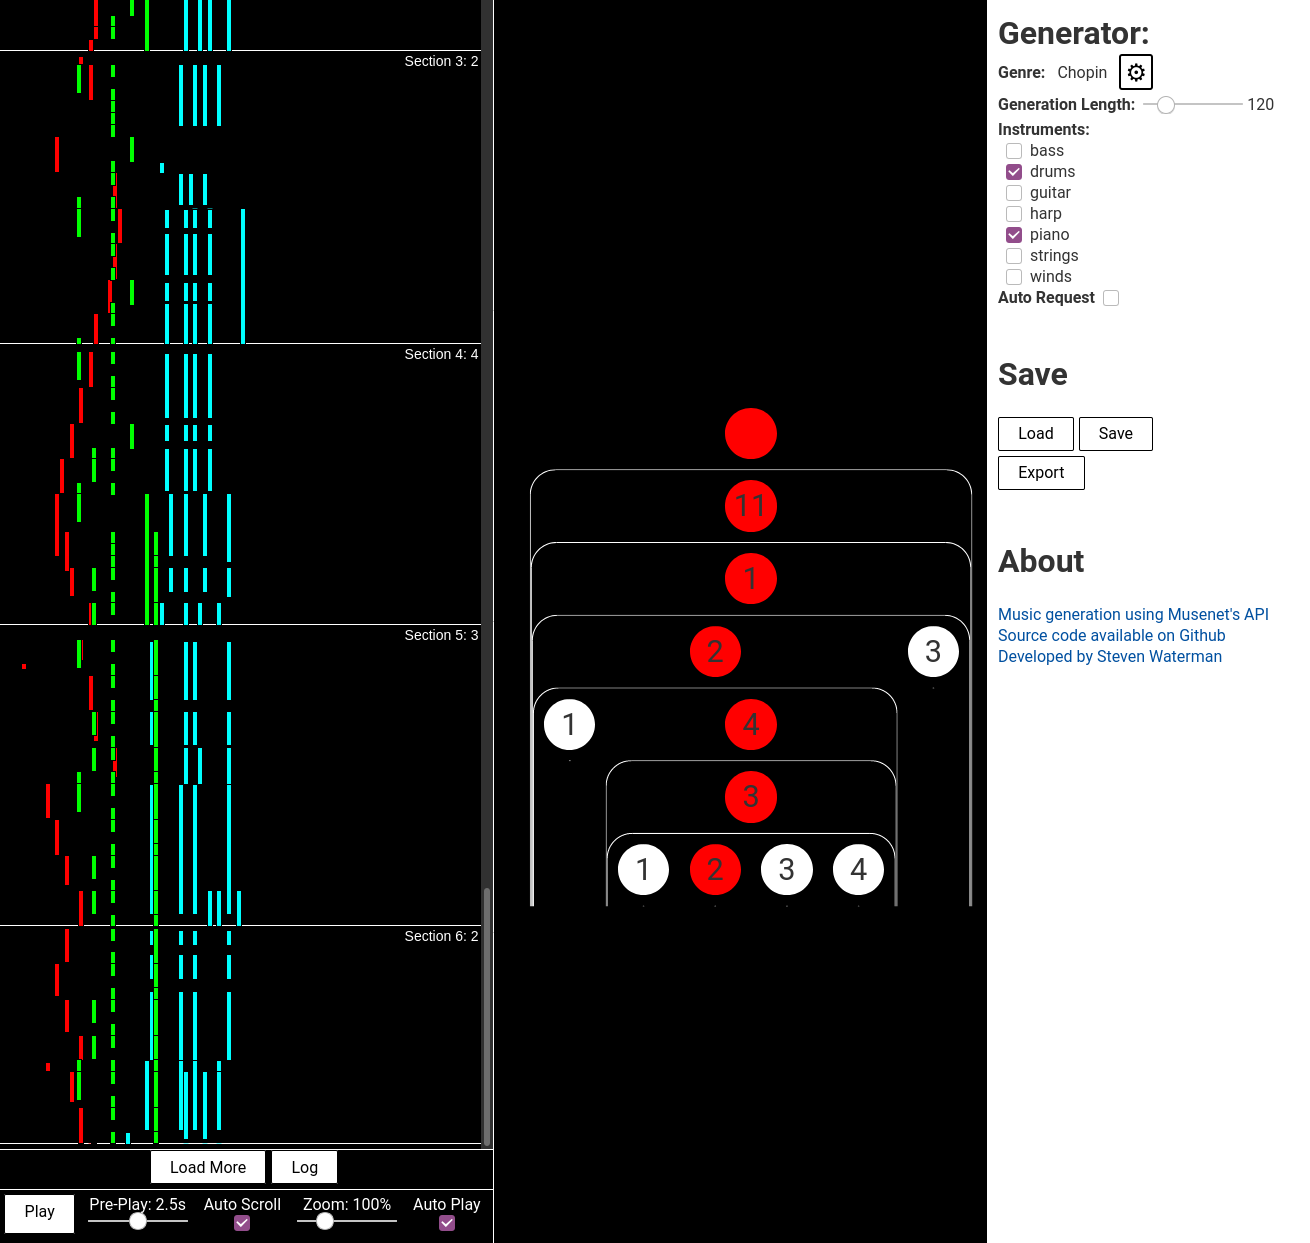
\includegraphics[width=0.9\linewidth]{musetree.png}}
		\end{center}
		\href{http://www.stevenwaterman.uk/musetree/}{\textbf{MuseTree} (Jan 2020)}
		
		A custom front-end for \href{https://openai.com/blog/musenet/}{MuseNet}, an AI music generator.
		Improves on the official MuseNet tool, turning a toy into something that can be used by creators in real-world scenarios.
		Successful open-source project, seeing frequent use in and contributions from the FOSS community.
		Latest update adds integration with the Web Audio API to perform real-time audio synthesis in-browser.
		
		\tech{Svelte} \tech{TypeScript} \tech{Web Audio}

		
		\begin{center}
			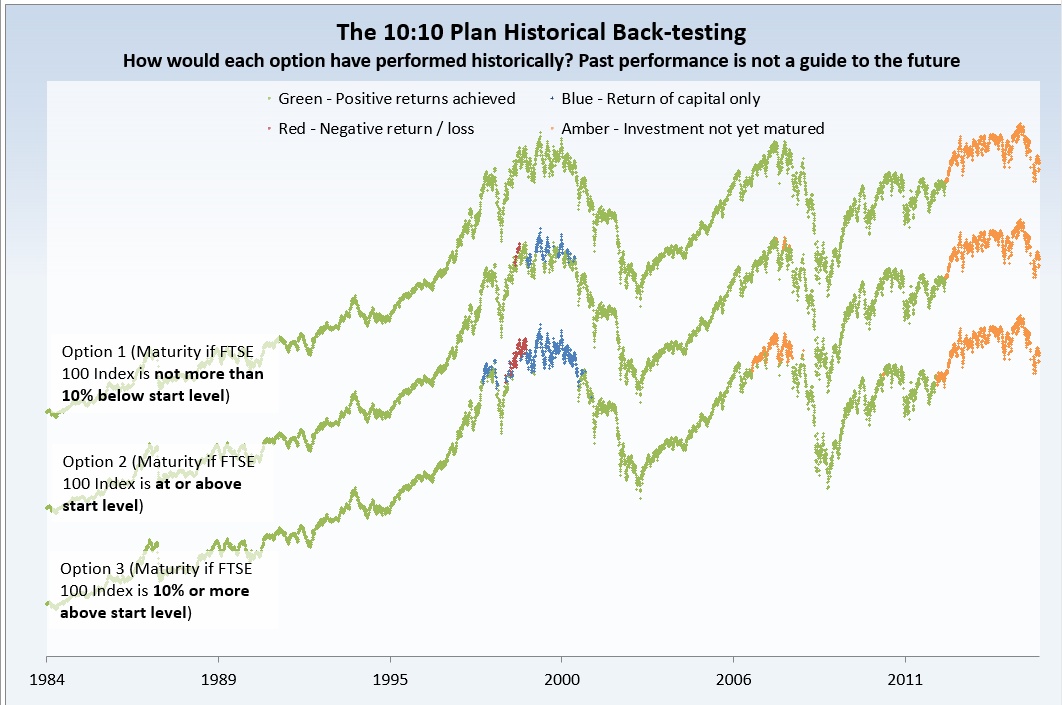
\includegraphics[width=0.9\linewidth]{backtest.png}
		\end{center}
		\vspace{-12pt}
		\textbf{Autocall Backtester} (March 2016)
		
		Created for Lowes Financial Management. Tests a financial product to see how it would have performed historically. This tool allowed the analysis to be performed where previously it was too time consuming. The graphs produced are used in the official product literature and online. The tool also informed the creation of new products, where backtesting revealed them to perform better than expected.
		
		\tech{Java} \tech{Excel} \tech{VBA}
		
		
	\end{minipage}
	\hspace{0.06\textwidth}
	\begin{minipage}{0.40\textwidth}	
		
		\begin{center}
			\href{https://github.com/stevenwaterman/sharpshot}{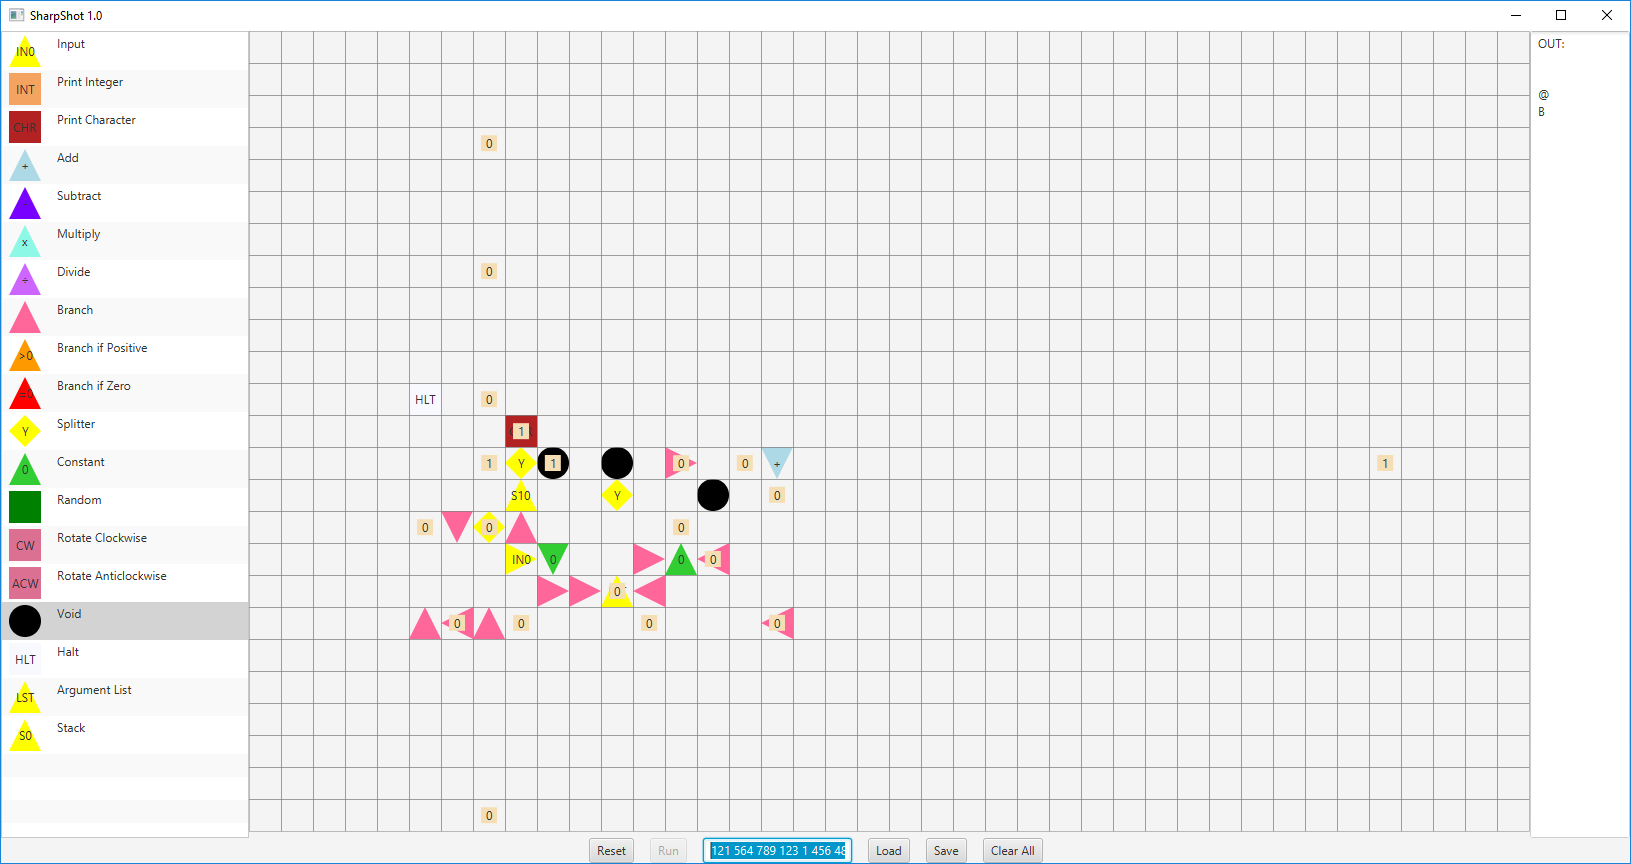
\includegraphics[width=0.9\linewidth]{sharpshot.png}}
		\end{center}
		\vspace{-12pt}
		\href{https://github.com/stevenwaterman/sharpshot}{\textbf{SharpShot} (Oct 2018)}
		
		Initial version created in 24 hours for \href{http://www.durhack.com}{Durhack 2018}. A visual, esoteric programming language where nodes are placed on a grid. Each node represents a function, and parameters move around the screen annihilating each other when they collide. SharpShot was the overall runner-up from 31 total projects, and won the GitHub prize for best Dev Tool. Work continued in 2019 to convert it into a Zachtronics-esque programming game.
		
		\tech{Java} \tech{Kotlin} \tech{Javafx}
		
		\begin{center}
			\href{http://www.dsurooms.com}{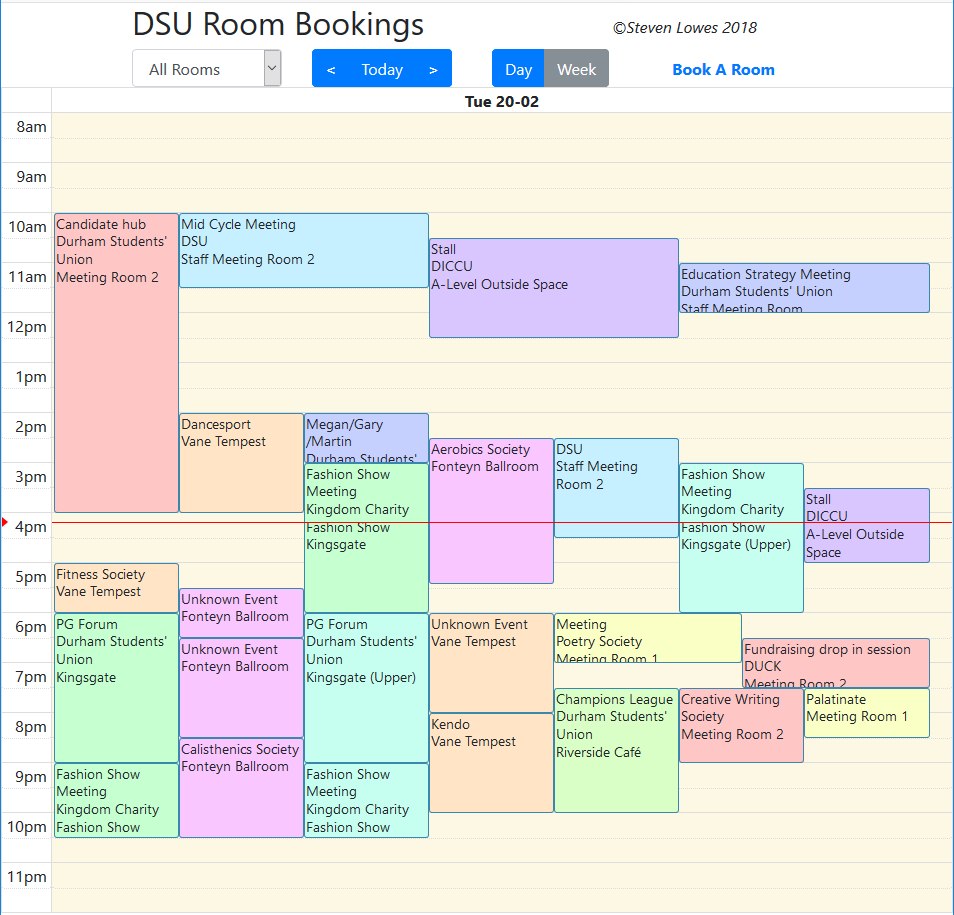
\includegraphics[width=0.9\linewidth]{dsurooms.png}}
		\end{center}
		\href{http://www.dsurooms.com}{\textbf{DSUrooms.com} (Jan 2018)}
		
		Created during my role in Student Group Governance, showing when rooms in the Students' Union were booked. Hosted in the cloud using a scraping API created with nodejs. Received very positive feedback from Student Groups, as previously there was no way to know which rooms were booked. The tool was successfully handed over to SU staff and is integrated into the official website.
		
		\tech{NodeJS} \tech{FullCalendar} \tech{Javascript} \tech{JQuery}
		
		
	\end{minipage}
	\hspace{0.02\textwidth}
\end{document}